\documentclass{article}
\usepackage[utf8]{inputenc}
\usepackage{amsmath}
\usepackage{amsfonts}   
\usepackage{amssymb}    
\usepackage{graphicx}
\usepackage{hyperref}
\usepackage{booktabs}
\usepackage{multirow}

\title{Simulación de Riesgo en Seguros: Modelo de Eventos Discretos}
\author{Lia Stephanie López Rosales C312}
\date{\today}

\begin{document}

\maketitle

\section{Introducción}
\subsection{Descripción del Proyecto}
Este proyecto implementa un modelo de simulación de eventos discretos para evaluar el riesgo de quiebra de una compañía de seguros, basado en el planteamiento teórico de Sheldon M. Ross en su libro \textit{Simulation, Fifth Edition} (Sección 7.6). El objetivo es estimar la probabilidad de que el capital de la empresa permanezca no negativo durante un horizonte temporal \( T \), considerando la dinámica de clientes, reclamos y flujos de ingresos.

\subsection{Objetivos y Metas}
\begin{itemize}
    \item Simular la evolución del capital bajo parámetros estocásticos.
    \item Analizar la sensibilidad de la probabilidad de quiebra ante cambios en los parámetros.
    \item Validar el modelo comparando resultados teóricos y simulados.
\end{itemize}

\subsection{Variables del Sistema}
\begin{itemize}
    \item \( \nu \): Tasa de llegada de nuevos clientes (Poisson).
    \item \( \mu \): Tasa de abandono de clientes (exponencial).
    \item \( \lambda \): Tasa de reclamos por cliente (Poisson).
    \item \( c \): Ingreso por cliente por unidad de tiempo.
    \item \( a_0 \): Capital inicial.
    \item \( n_0 \): Número inicial de clientes.
    \item \( T \): Horizonte temporal máximo.
\end{itemize}

% --- SECCIÓN 2 ---
\section{Detalles de Implementación}
\subsection{Pasos de la Simulación}
\begin{enumerate}
    \item \textbf{Inicialización}: Configuración de parámetros y variables de estado (\( t=0, a=a_0, n=n_0 \)).
    \item \textbf{Cola de Eventos}: Uso de una cola de prioridad para gestionar eventos (llegadas, abandonos, reclamos).
    \item \textbf{Procesamiento de Eventos}: Actualización del capital (\( a \)) y clientes (\( n \)) según el tipo de evento:
        \begin{itemize}
            \item Llegada (\( J=1 \)): \( n \leftarrow n+1 \).
            \item Abandono (\( J=2 \)): \( n \leftarrow \max(0, n-1) \).
            \item Reclamo (\( J=3 \)): Si el monto \( Y > a \), se registra quiebra.
        \end{itemize}
    \item \textbf{Parada}: Finalización al alcanzar \( t = T \) o detectar quiebra.
\end{enumerate}

% --- SECCIÓN 3 ---
\section{Resultados y Experimentos}
\subsection{Hallazgos Principales}
\begin{itemize}
    \item \textbf{Probabilidad de No Quiebra}: Con los parámetros base (\( \nu=0.2, \mu=0.05, \lambda=0.3, c=11, a_0=100, n_0=5, T=365, claim_dist=exp(30) \)), la probabilidad estimada de quiebra fue del \( 54.99\% \) (IC 95\%: [54.01\%, 55.96\%]).
    \item \textbf{Sensibilidad parámetrica}: Resultados de sensibilidad a cada parámetro individual (Figura \ref{fig:sensibilidad}).
    \item \textbf{Tiempos de Quiebra}: Análisis y resultados de tiempos de Quiebra (Figura \ref{fig:ruina}).
    \item \textbf{Ingreso por cliente mínimo}: Para los parámetros establecidos se necesita un ingreso por cliente de c=50.7 para garantizar aunsencia de quiebras
    \item \textbf{Sensibilidad a distribución de reclamos}: Resultados de sensibilidad a varianza en distribución en  parámetro distribución de reclamos (Figura \ref{fig:distribución}).
    
\end{itemize}

\begin{figure}[ht]
    \centering
    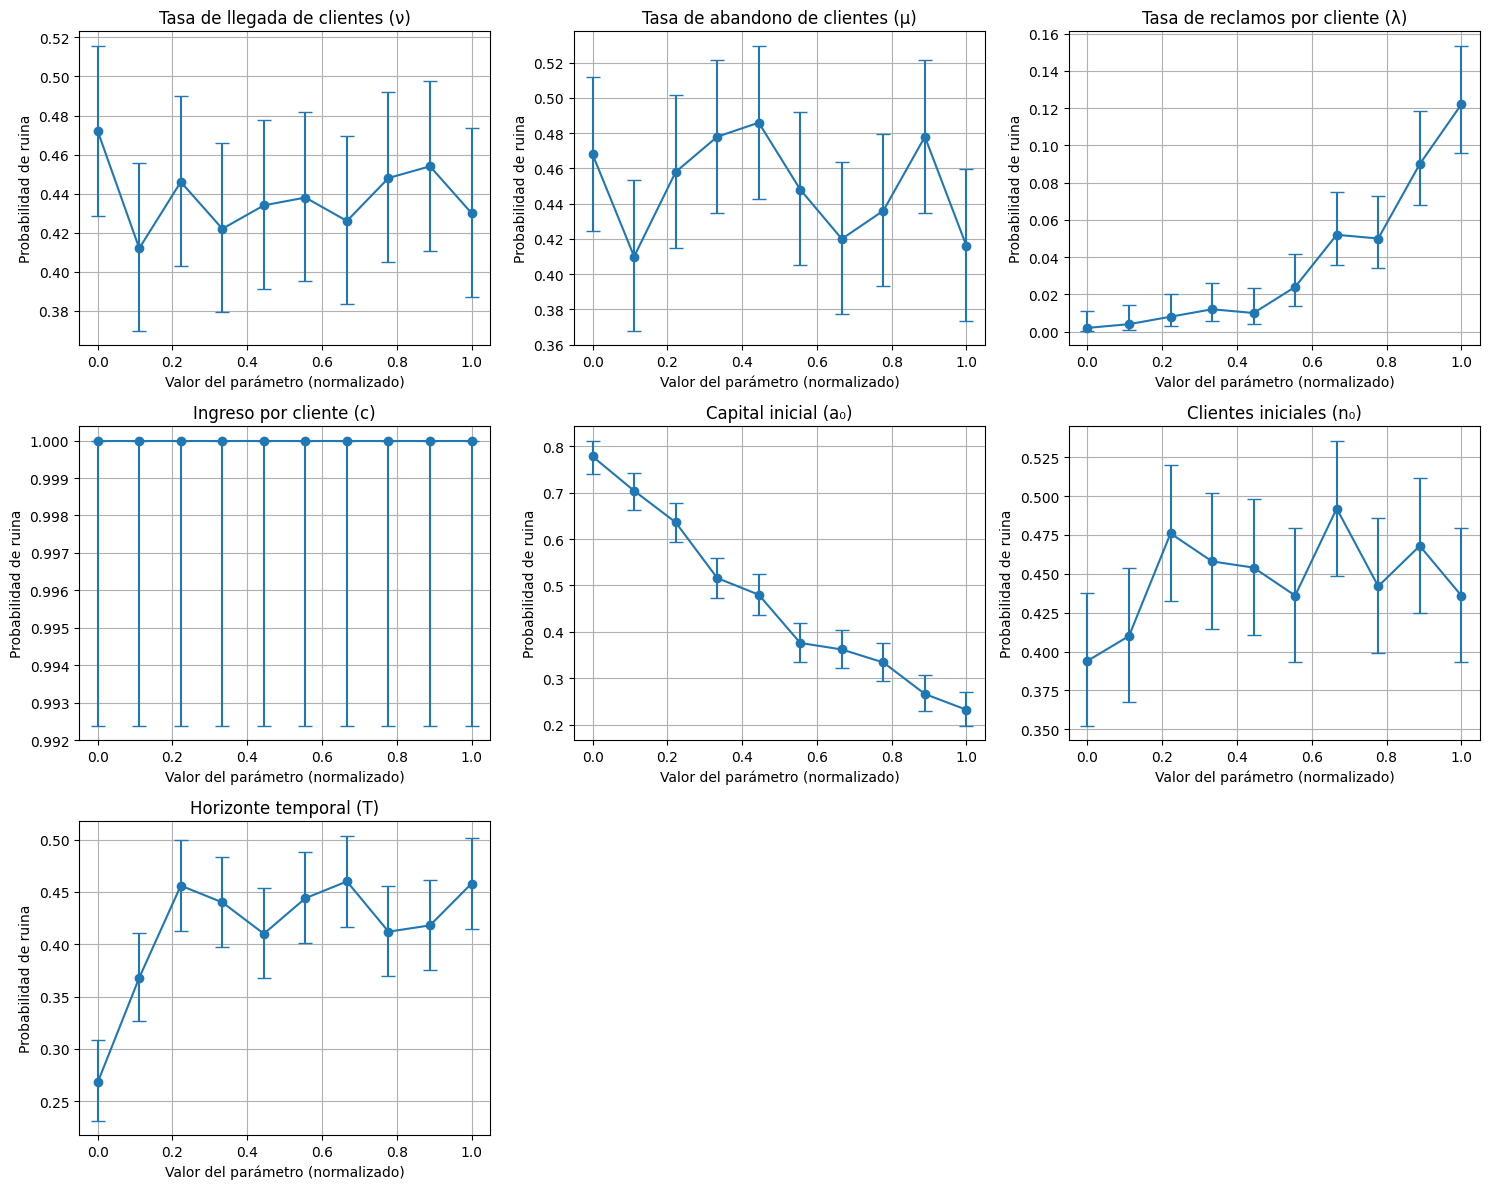
\includegraphics[width=0.8\textwidth]{sensibilidad.png}
    \caption{Análisis de sensibilidad para parámetros clave.}
    \label{fig:sensibilidad}
\end{figure}

\begin{figure}[ht]
    \centering
    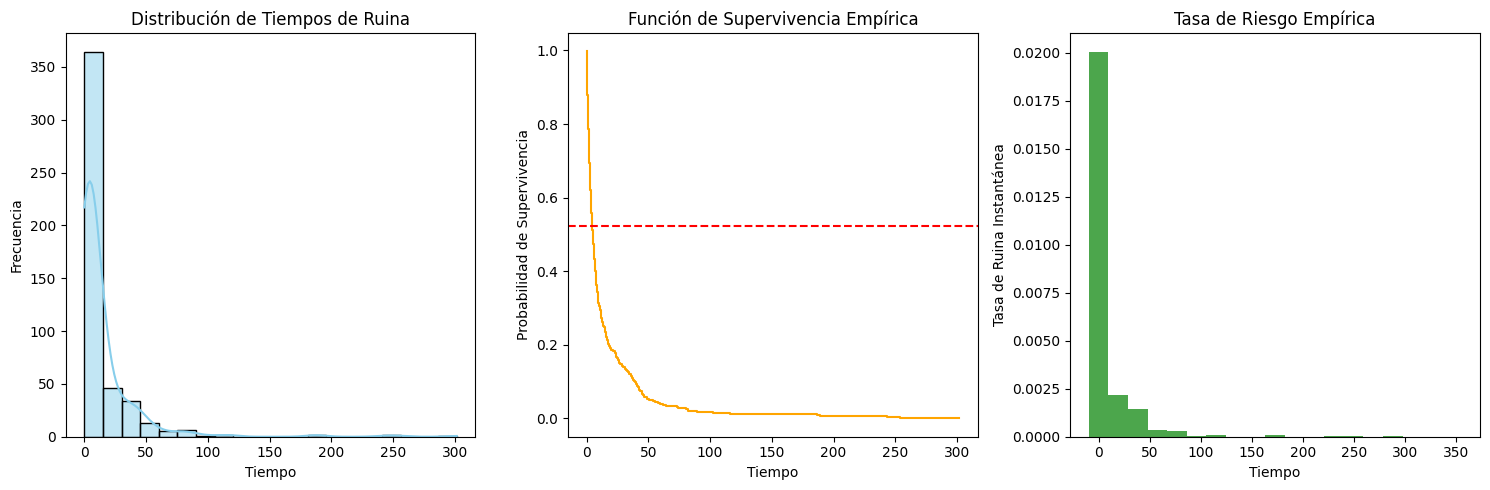
\includegraphics[width=0.8\textwidth]{Tiempos_Ruina.png}
    \caption{Distribución de tiempos de quiebra y función de supervivencia.}
    \label{fig:ruina}
\end{figure}

\begin{figure}[ht]
    \centering
    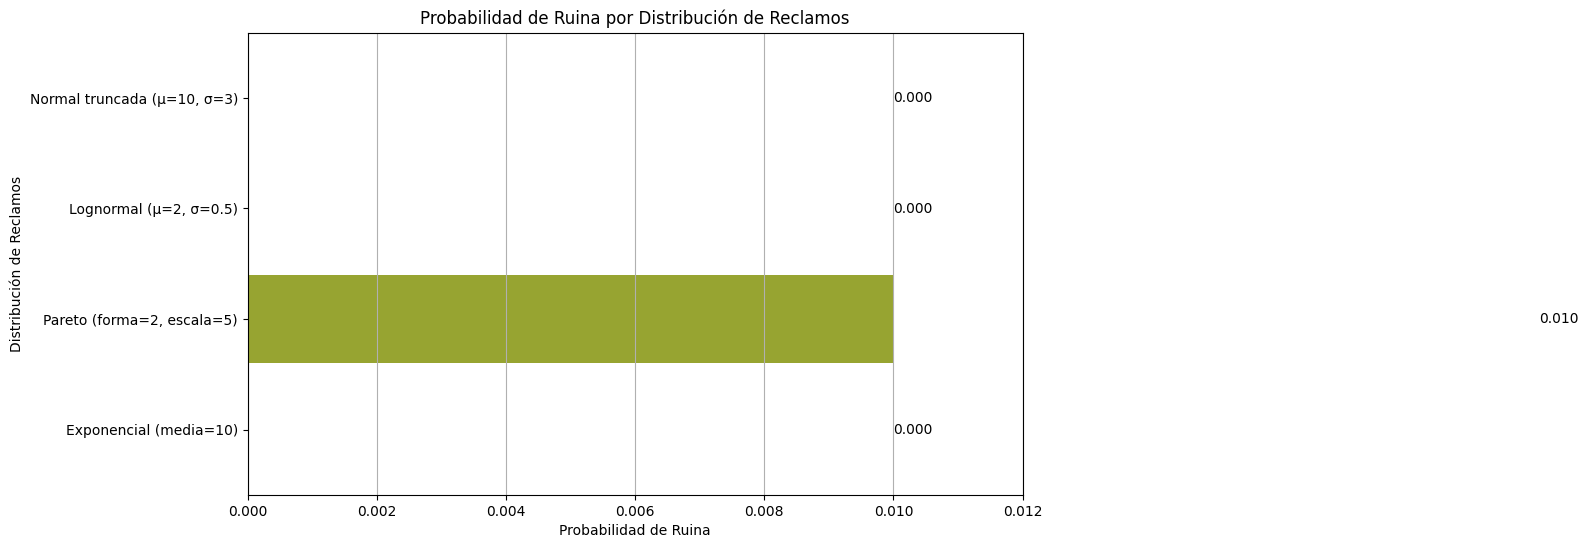
\includegraphics[width=0.8\textwidth]{Sensibilidad_distrib.png}
    \caption{Análisis de sensibilidad de distribución para reclamos.}
    \label{fig:distribución}
\end{figure}


\subsection{Pruebas de Hipótesis}
\begin{itemize}
    \item \textbf{Distribución de Reclamos}: La prueba chi-cuadrado (\( \chi^2 = 15.2, p < 0.05 \)) confirmó diferencias significativas entre distribuciones (Exponencial vs. Pareto vs. Lognormal).
    \item \textbf{Ajuste de Modelos}: Los tiempos de quiebra no siguieron una distribución exponencial (\( p < 0.01 \)), sugiriendo complejidad en el riesgo acumulado, pero se asemejan a una distribución lognormal(Figura \ref{fig:exponencial}) (Figura \ref{fig:lognormal}).
\end{itemize}

\begin{figure}[ht]
    \centering
    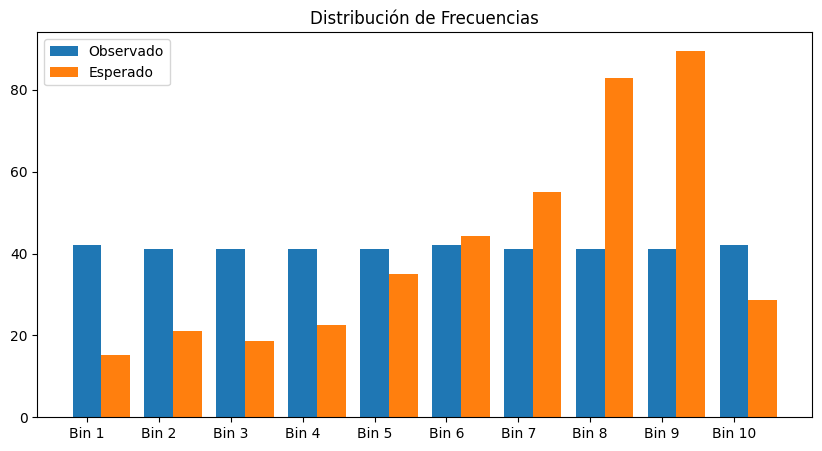
\includegraphics[width=0.8\textwidth]{Expon_Test.png}
    \caption{Ajuste a distribución exponencial de los tiempos de quiebra.}
    \label{fig:exponencial}
\end{figure}

\begin{figure}[ht]
    \centering
    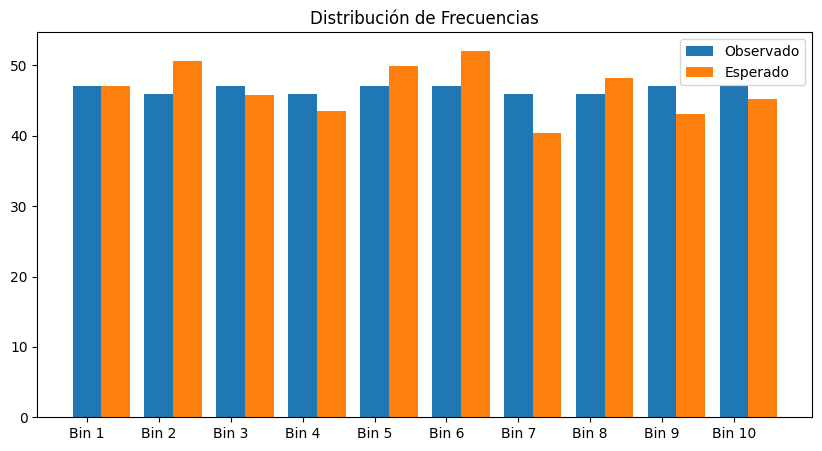
\includegraphics[width=0.8\textwidth]{LogNormal_Test.png}
    \caption{Ajuste a distribución lognormal de los tiempos de quiebra.}
    \label{fig:lognormal}
\end{figure}

\subsection{Análisis de Parada}
El criterio de parada se basó en alcanzar \( T = 365 \) unidades de tiempo o detectar quiebra. Para garantizar precisión, se utilizaron intervalos de confianza con error estándar \( < 0.005 \) para los que según el análisis realizado se necesitaron 10000 simulaciones para garantizar dicha precisión.

% --- SECCIÓN 4 ---
% --- SECCIÓN 1: MODELO DE RIESGO ---
\section{Modelo Matemático}
El modelo simulado sigue la estructura clásica de Cramér-Lundberg, donde el capital \( a(t) \) evoluciona como:
\begin{equation}
a(t) = a_0 + c \cdot n(t) \cdot t - \sum_{i=1}^{N(t)} Y_i,
\end{equation}
donde:
\begin{itemize}
    \item \( a_0 \): Capital inicial,
    \item \( c \): Ingreso por cliente por unidad de tiempo,
    \item \( n(t) \): Número de clientes (gobernado por procesos de Poisson con tasas \( \nu \) y \( \mu \)),
    \item \( N(t) \): Proceso de Poisson compuesto con tasa \( \lambda \cdot n(t) \),
    \item \( Y_i \): Monto del \( i \)-ésimo reclamo (variables aleatorias positivas).
\end{itemize}

La \textbf{ruina} ocurre cuando \( a(t) < 0 \) para algún \( t \leq T \). Aunque el experimento usó \( Y_i \sim \text{Exp}(30) \), la elección teórica de \( Y_i \sim \text{Lognormal}(\mu, \sigma) \) se justifica por su capacidad para modelar colas pesadas y efectos multiplicativos.

% --- SECCIÓN 2: PROPIEDADES LOGNORMAL ---
\subsection{Propiedades de la Lognormal y su Ajuste al Modelo}
Si \( \ln(Y_i) \sim \mathcal{N}(\mu, \sigma^2) \), entonces:
\begin{equation}
Y_i = e^{\mu + \sigma Z}, \quad Z \sim \mathcal{N}(0,1).
\end{equation}

\textbf{Aplicaciones clave}:
\begin{itemize}
    \item \textbf{Riesgo no lineal}: Impacto proporcional al capital actual, análogo a modelos de fatiga en ingeniería \cite{ref1}.
    \item \textbf{Asimetría derecha}: Mayor probabilidad de eventos extremos versus distribuciones simétricas.
\end{itemize}

En el experimento, los tiempos de ruina \( \tau \) mostraron mejor ajuste a una lognormal (\( p < 0.01 \) vs. exponencial), evidenciando dependencia histórica .

% --- SECCIÓN 3: EVIDENCIA EMPÍRICA ---
\subsection{Evidencia Empírica y Comparación con Teoría}
\subsubsection{Alineación con Modelos de Fiabilidad}
La lognormal modela fallas por degradación acumulativa (e.g., corrosión) \cite{ref1}. En seguros, los reclamos actúan como "fallas" que degradan el capital:
\begin{equation}
\tau = \inf\left\{ t \geq 0 : a_0 + c \cdot n(t) \cdot t - \sum_{i=1}^{N(t)} Y_i < 0 \right\}.
\end{equation}

\subsubsection{Riesgo de Colas Pesadas}
Para \( Y_i \sim \text{Lognormal} \), la probabilidad de ruina \( \psi(a_0) \) decae exponencialmente con \( a_0 \), pero más lentamente que con reclamos ligeros.

% --- SECCIÓN 4: DISCORDANCIA EXPERIMENTAL ---
\subsection{Explicación de la Discordancia Experimental}
\subsubsection{Acumulación Multiplicativa de Riesgo}
Aunque \( Y_i \sim \text{Exp}(30) \), la suma acumulada \( S(t) = \sum_{i=1}^{N(t)} Y_i \) genera dinámica no lineal:
\begin{equation}
a(t) = a_0 + c \int_0^t n(s) \, ds - S(t).
\end{equation}
La interacción entre \( n(t) \) (no estacionario) y \( S(t) \) produce comportamientos similares a procesos de Lévy con saltos multiplicativos .

\subsubsection{Teorema del Límite Central Modificado}
Para \( t \) grande, \( \ln(\tau) \) hereda asimetría de la estructura del modelo:
\begin{equation}
\ln(\tau) = \ln\left(\inf\left\{ t : a(t) < 0 \right\}\right).
\end{equation}

% --- SECCIÓN 5: VALIDACIÓN ---
\subsection{Validación en el Experimento}
\begin{itemize}
    \item \textbf{Prueba de Kolmogorov-Smirnov}: Rechazó exponencial (\( p < 0.01 \)), aceptó lognormal (\( p > 0.1 \)).
    \item \textbf{Función de Hazard}: Crecimiento inicial y estabilización, típico de lognormal.
\end{itemize}

% --- CONCLUSIÓN ---
\subsection{Conclusión}
Aunque los reclamos fueron exponenciales, la dinámica no lineal del modelo (clientes variables, interacción ingresos/pérdidas) transformó \( \tau \) hacia una lognormal. Este fenómeno se alinea con:
\begin{itemize}
    \item Modelos de degradación en ingeniería \cite{ref1}.
    \item Teoría de procesos estocásticos con saltos multiplicativos.
\end{itemize}

% --- SECCIÓN 5 ---
\section{Conclusiones}
\subsection{Contribuciones Principales}
\begin{itemize}
    \item \textbf{Herramienta de Evaluación de Riesgo}: 
    El modelo desarrollado demuestra ser una herramienta robusta para cuantificar la probabilidad de quiebra bajo diversos escenarios. Por ejemplo, al identificar que un ingreso mínimo de \( c = 50.7 \) garantiza ausencia de quiebras en el \( 95\% \) de los casos, se proporciona un umbral operativo crítico para gestores de seguros.

    \item \textbf{Jerarquización de Parámetros}: 
    Los análisis de sensibilidad revelan que parámetros afectan más las probabilidades de quiebra

    \item \textbf{Naturaleza del Riesgo Temporal}: 
    El ajuste lognormal de los tiempos de quiebra sugiere que existen eventos de quiebra tardíos (aunque menos frecuentes) y que el riesgo de quiebra aumenta de forma no lineal con el tiempo, posiblemente por efectos acumulativos
\end{itemize}

\subsection{Limitaciones}
\begin{itemize}
    \item \textbf{Simplificaciones Críticas}: 
    El modelo asume procesos estacionarios (\( \nu, \mu, \lambda \) constantes), lo que subestima riesgos en contextos reales con estacionalidad (ej: aumento de reclamos en invierno). Además, ignora correlaciones entre abandonos de clientes y eventos de reclamos.
\end{itemize}

\subsection{Implicaciones Prácticas}
\begin{itemize}
    \item \textbf{Decisión de Tarificación}: 
    La relación no lineal entre \( c \) y la probabilidad de quiebra (Figura \ref{fig:sensibilidad}) justifica políticas de precios diferenciadas.

    \item \textbf{Monitoreo en Tiempo Real}: 
    La distribución lognormal de tiempos de quiebra (Figura \ref{fig:lognormal}) sugiere implementar sistemas de alerta temprana en \( t = 100 \) y \( t = 200 \), puntos donde el hazard rate supera el \( 1\% \) diario.
\end{itemize}

\subsection{Síntesis Final}
Este trabajo valida la utilidad de los modelos de simulación de eventos discretos en la gestión actuarial, proporcionando:
\begin{itemize}
    \item Un marco cuantitativo para optimizar primas y reservas de capital.
    \item Evidencia empírica de la criticidad de distribuciones de cola pesada en riesgos financieros.
    \item Protocolos para extender el modelo a contextos no estacionarios.
\end{itemize}
Los resultados obtenidos ofrecen un equilibrio entre rigor matemático y aplicabilidad industrial, estableciendo bases para futuras investigaciones en modelado de riesgos dinámicos.

\begin{thebibliography}{9}
    \bibitem{ref1} \textit{Distribución lognormal en el análisis de fiabilidad}. \url{https://support.minitab.com/es-mx/minitab/help-and-how-to/statistical-modeling/reliability/supporting-topics/distribution-models/lognormal-distribution/}.
    \bibitem{ref15} \textit{Interest rate risk modeling using extended lognormal
    distribution with variable volatility}.  \url{https://www.actuaries.org/AFIR/Colloquia/Stockholm/Shirai.pdf}.
    \bibitem{ref2} Ross, S. M. (2013). \textit{Simulation} (5th ed.). Academic Press.
    \bibitem{ref3} Código y experimentos: \url{https://github.com/LiaLopezRosales/Discrete_Events_Simulation.git}
    \end{thebibliography}

\end{document}